\documentclass[11pt,letterpaper]{article}

\usepackage[margin=1in]{geometry}
\usepackage{graphicx}
\usepackage{subcaption}
\usepackage{booktabs}
\usepackage{hyperref}
\usepackage{parskip}
\usepackage{float}
\usepackage{microtype}
\usepackage{amsmath}

\hypersetup{colorlinks=true, linkcolor=blue, urlcolor=blue}

\title{\textbf{CS5330 Computer Vision: Project 2}\\
       \large Content-Based Image Retrieval}
\author{Shriman Raghav Srinivasan \and Shyam Sreenivasan}
\date{June 2026}

\begin{document}

\maketitle

% ============================================================
\section*{Project Overview}
% ============================================================

For this project we built a content-based image retrieval (CBIR) system in C++.
The idea is simple: given a target image and a database of images, find the ones
that look most similar to the target. We implemented seven different ways of doing
this, ranging from a basic pixel patch comparison to deep network embeddings from
a pre-trained ResNet18 model.

The classic methods each describe an image as a feature vector, either the raw
pixel values in a small patch, a color histogram, a grid of spatial histograms, or
a combination of a color histogram and a texture histogram built from Sobel gradient
magnitudes. The deep method reads pre-computed 512-dimensional embeddings from a CSV
file and uses cosine distance to find semantically similar images. We also built a
custom method that combines color histograms with DNN embeddings to get the best of
both worlds.

All feature extraction and distance computation is written in C++. The entire system
runs as a single command-line program that takes a target image, a database directory,
a method name, and the number of results N to return.

We split the tasks: Shyam implemented Tasks 1 through 3 (baseline, histogram, and
multi-histogram matching). Shriman implemented Tasks 4 through 7 (texture and color,
DNN embeddings, comparison analysis, and the custom design).

% ============================================================
\section*{Source Code}
% ============================================================

The full source code for this project is available at:\\
\url{https://github.com/shyams612/CS5330-Computer-Vision/tree/main/Projects/project2}

% ============================================================
\section*{Results}
% ============================================================

%------------------------------------------------------------
\subsection*{Task 1: Baseline Matching (7x7 Center Patch + SSD)}
%------------------------------------------------------------

We extract the 7x7 pixel patch centered in each image (147 BGR values) and use
Sum of Squared Differences (SSD) as the distance metric. A score of 0 means
the patches are identical. This is a simple but surprisingly effective baseline
for images where the central subject is similar.

\begin{figure}[H]
    \centering
    \begin{subfigure}[b]{0.18\textwidth}
        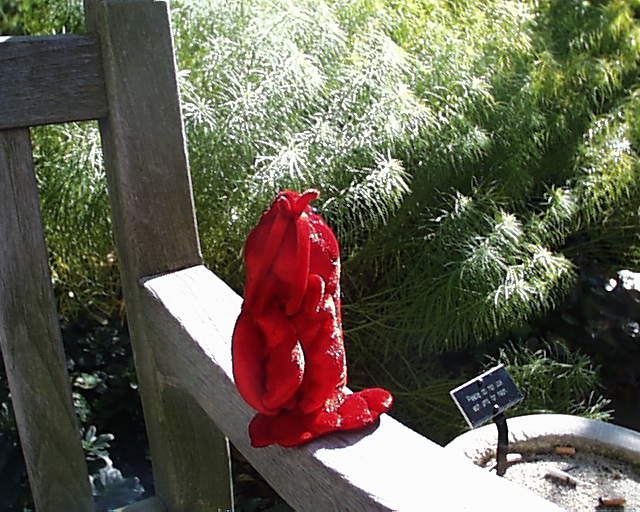
\includegraphics[width=\textwidth]{report_imgs/pic.1016.jpg}
        \caption{Target\\pic.1016}
    \end{subfigure}
    \hfill
    \begin{subfigure}[b]{0.18\textwidth}
        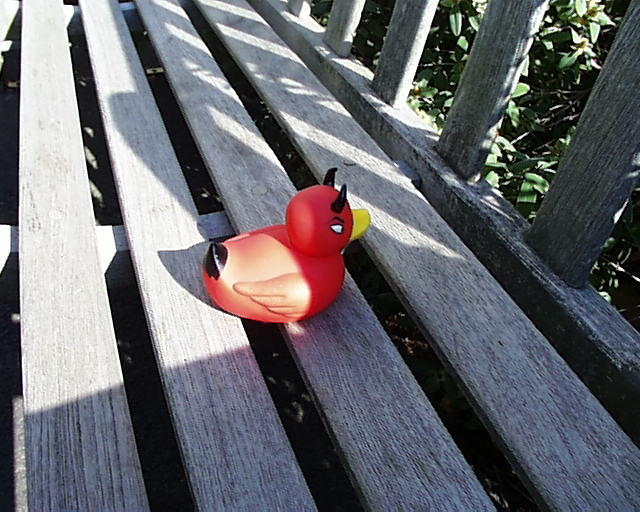
\includegraphics[width=\textwidth]{report_imgs/pic.0986.jpg}
        \caption{Match 1\\pic.0986\\SSD: 14049}
    \end{subfigure}
    \hfill
    \begin{subfigure}[b]{0.18\textwidth}
        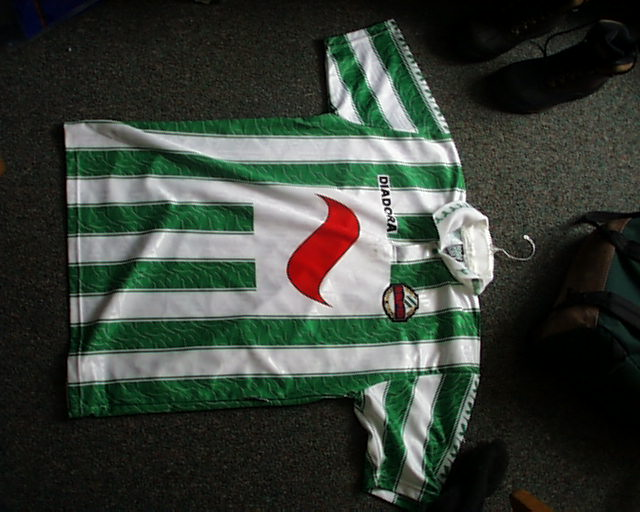
\includegraphics[width=\textwidth]{report_imgs/pic.0641.jpg}
        \caption{Match 2\\pic.0641\\SSD: 21756}
    \end{subfigure}
    \hfill
    \begin{subfigure}[b]{0.18\textwidth}
        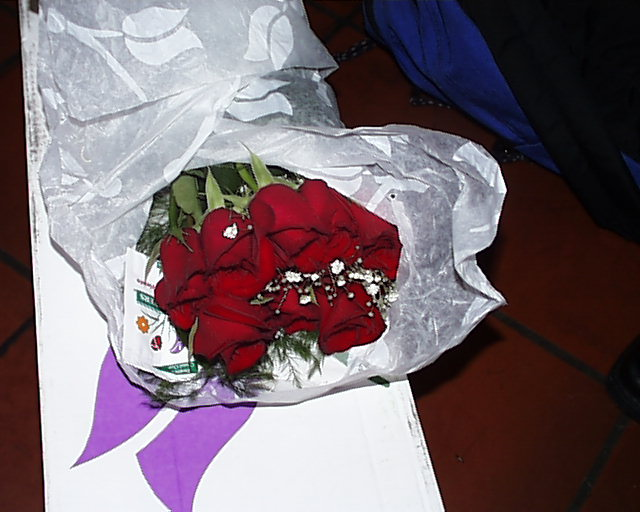
\includegraphics[width=\textwidth]{report_imgs/pic.0547.jpg}
        \caption{Match 3\\pic.0547\\SSD: 49703}
    \end{subfigure}
    \caption{Task 1: Top 3 matches for \texttt{pic.1016.jpg} using the 7x7 center
    patch and SSD distance. The matches agree with the expected results from the
    assignment spec. All matched images share similar central pixel colors to
    the target.}
\end{figure}

%------------------------------------------------------------
\subsection*{Task 2: Histogram Matching (3D Color Histogram + Intersection)}
%------------------------------------------------------------

We compute a 3D BGR histogram over the whole image with 16 bins per channel
(4096 total bins), normalize it by pixel count, and use histogram intersection
as the distance metric. Intersection is negated so that lower scores mean more
similar images. A score of $-1$ means the histograms are identical.

\begin{figure}[H]
    \centering
    \begin{subfigure}[b]{0.22\textwidth}
        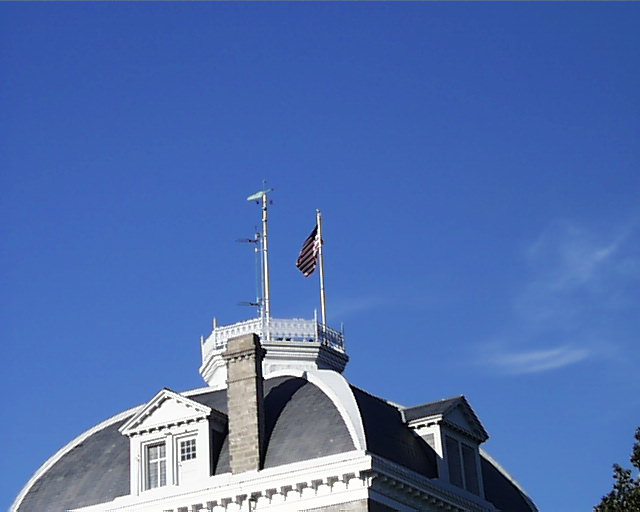
\includegraphics[width=\textwidth]{report_imgs/pic.0164.jpg}
        \caption{Target\\pic.0164}
    \end{subfigure}
    \hfill
    \begin{subfigure}[b]{0.22\textwidth}
        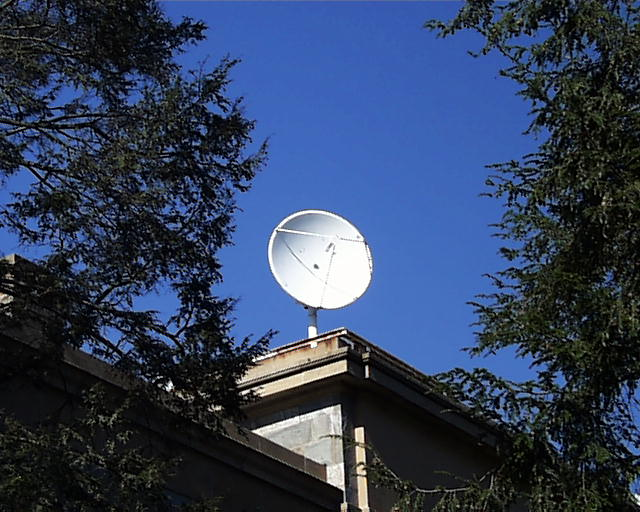
\includegraphics[width=\textwidth]{report_imgs/pic.0110.jpg}
        \caption{Match 1\\pic.0110\\score: $-0.389$}
    \end{subfigure}
    \hfill
    \begin{subfigure}[b]{0.22\textwidth}
        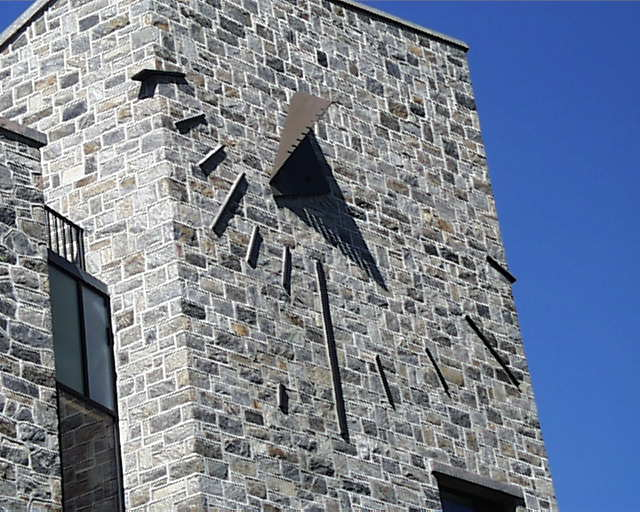
\includegraphics[width=\textwidth]{report_imgs/pic.0092.jpg}
        \caption{Match 2\\pic.0092\\score: $-0.361$}
    \end{subfigure}
    \hfill
    \begin{subfigure}[b]{0.22\textwidth}
        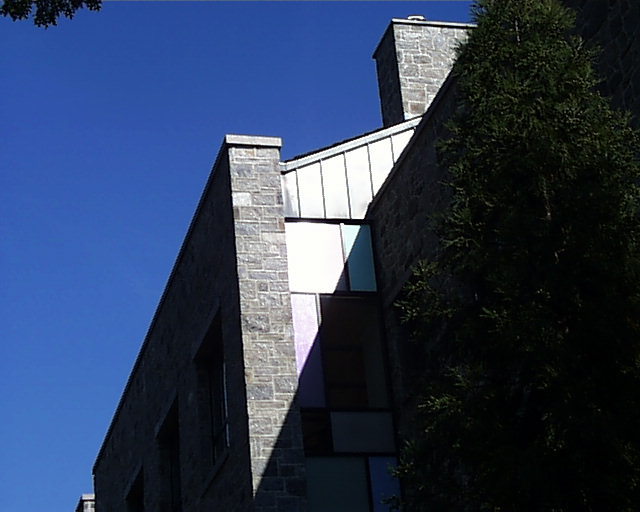
\includegraphics[width=\textwidth]{report_imgs/pic.1032.jpg}
        \caption{Match 3\\pic.1032\\score: $-0.337$}
    \end{subfigure}
    \caption{Task 2: Top 3 matches for \texttt{pic.0164.jpg} using a 3D BGR
    histogram with 16 bins per channel and histogram intersection. The results
    make sense: all matched images share a similar overall color distribution
    to the target, likely dominated by the same dominant hue range.}
\end{figure}

%------------------------------------------------------------
\subsection*{Task 3: Multi-Histogram Matching (3x3 Spatial Grid)}
%------------------------------------------------------------

We divide each image into a 3x3 grid of 9 non-overlapping regions. For each
region we compute a normalized 3D BGR histogram with 8 bins per channel (512
values per region, 4608 total). We compare corresponding regions using histogram
intersection and average the 9 region scores with equal weights. This spatial
layout captures where colors appear in the image, not just what colors appear.

\begin{figure}[H]
    \centering
    \begin{subfigure}[b]{0.22\textwidth}
        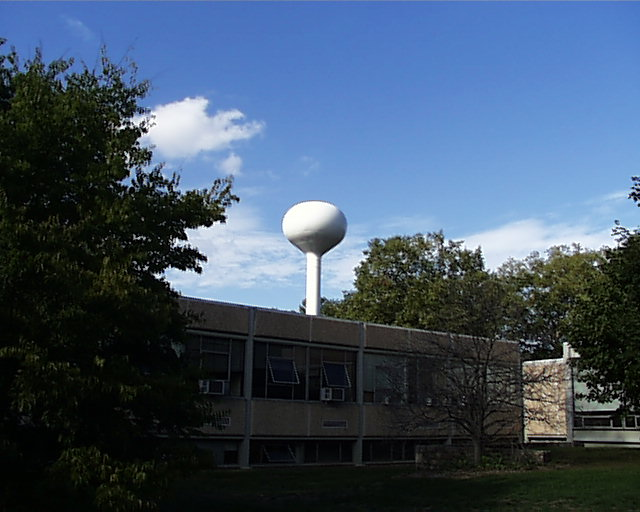
\includegraphics[width=\textwidth]{report_imgs/pic.0274.jpg}
        \caption{Target\\pic.0274}
    \end{subfigure}
    \hfill
    \begin{subfigure}[b]{0.22\textwidth}
        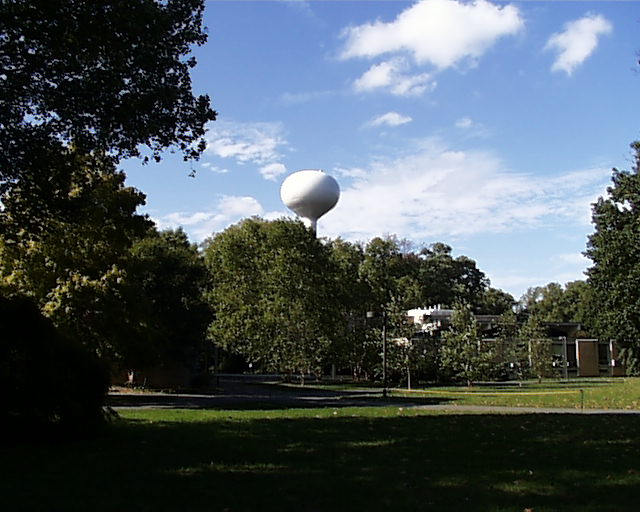
\includegraphics[width=\textwidth]{report_imgs/pic.0273.jpg}
        \caption{Match 1\\pic.0273\\score: $-0.571$}
    \end{subfigure}
    \hfill
    \begin{subfigure}[b]{0.22\textwidth}
        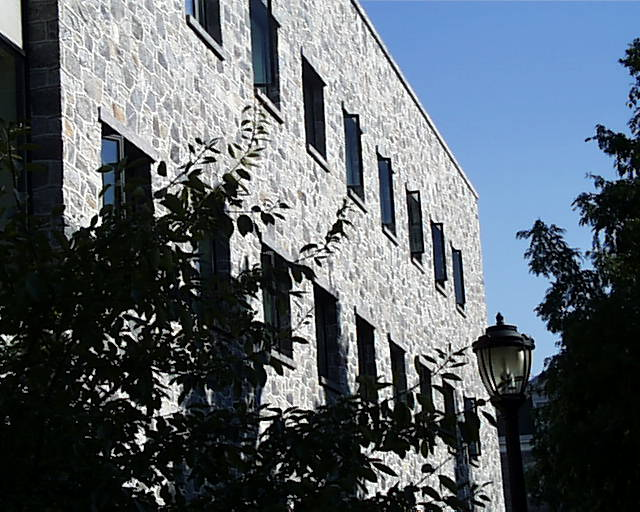
\includegraphics[width=\textwidth]{report_imgs/pic.1031.jpg}
        \caption{Match 2\\pic.1031\\score: $-0.520$}
    \end{subfigure}
    \hfill
    \begin{subfigure}[b]{0.22\textwidth}
        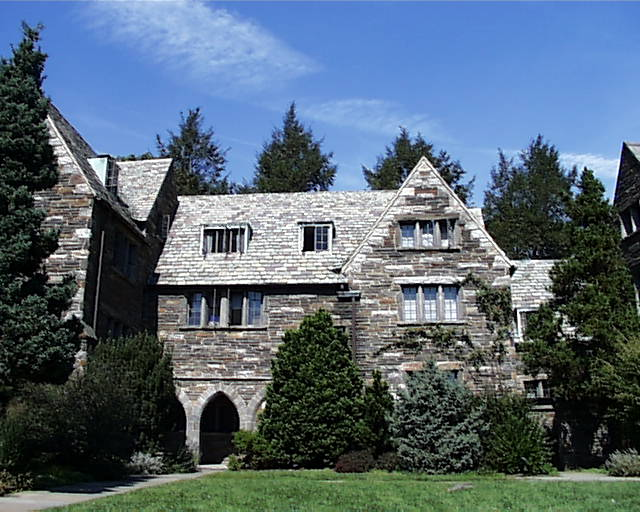
\includegraphics[width=\textwidth]{report_imgs/pic.0409.jpg}
        \caption{Match 3\\pic.0409\\score: $-0.518$}
    \end{subfigure}
    \caption{Task 3: Top 3 matches for \texttt{pic.0274.jpg} using a 3x3
    spatial grid of BGR histograms with equal region weights. The results make
    sense: pic.0273 is nearly identical (likely a sequential shot of the same
    scene), and the other matches share similar sky-to-ground color layout as
    the target.}
\end{figure}

%------------------------------------------------------------
\subsection*{Task 4: Texture and Color}
%------------------------------------------------------------

We concatenate two normalized histograms as the feature vector. The color part
is a whole-image 3D BGR histogram with 8 bins per channel (512 values). The
texture part is a Sobel gradient magnitude histogram with 16 bins (16 values).
The Sobel kernels are applied manually from scratch on a manual grayscale
conversion -- no \texttt{cv::Sobel} or \texttt{cv::calcHist} used. Each pixel's
gradient magnitude $M = \sqrt{G_x^2 + G_y^2}$ is binned into 16 equally spaced
bins across the range $[0, \sqrt{2} \cdot 4 \cdot 255]$.

The distance metric computes histogram intersection on each sub-histogram
independently and averages them with equal weight:
\[
D = -\bigl(0.5 \cdot \text{colorIntersect} + 0.5 \cdot \text{textureIntersect}\bigr)
\]

\begin{figure}[H]
    \centering
    \begin{subfigure}[b]{0.22\textwidth}
        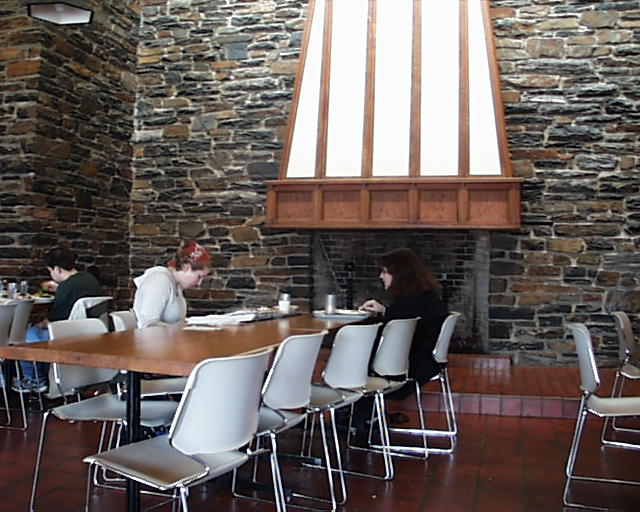
\includegraphics[width=\textwidth]{report_imgs/pic.0535.jpg}
        \caption{Target\\pic.0535}
    \end{subfigure}
    \hfill
    \begin{subfigure}[b]{0.22\textwidth}
        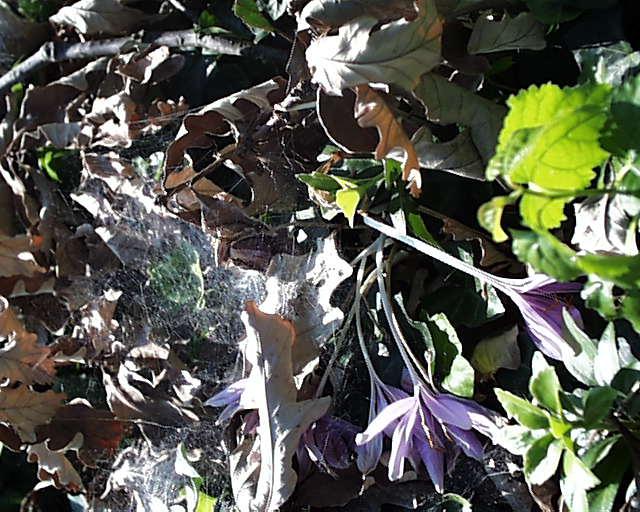
\includegraphics[width=\textwidth]{report_imgs/pic.0853.jpg}
        \caption{Match 1\\pic.0853\\score: $-0.826$}
    \end{subfigure}
    \hfill
    \begin{subfigure}[b]{0.22\textwidth}
        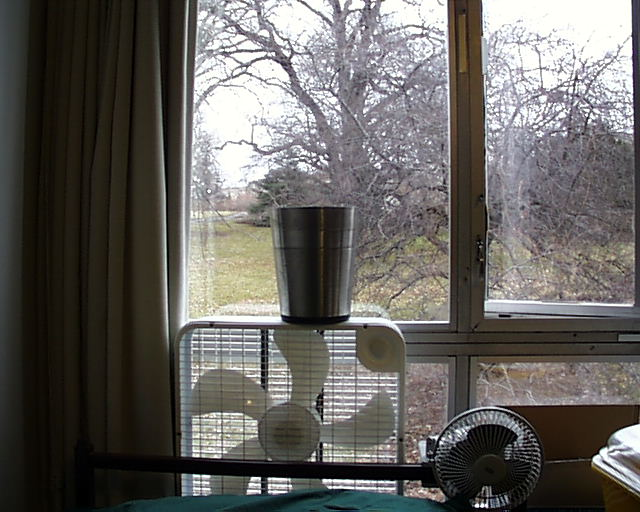
\includegraphics[width=\textwidth]{report_imgs/pic.0605.jpg}
        \caption{Match 2\\pic.0605\\score: $-0.825$}
    \end{subfigure}
    \hfill
    \begin{subfigure}[b]{0.22\textwidth}
        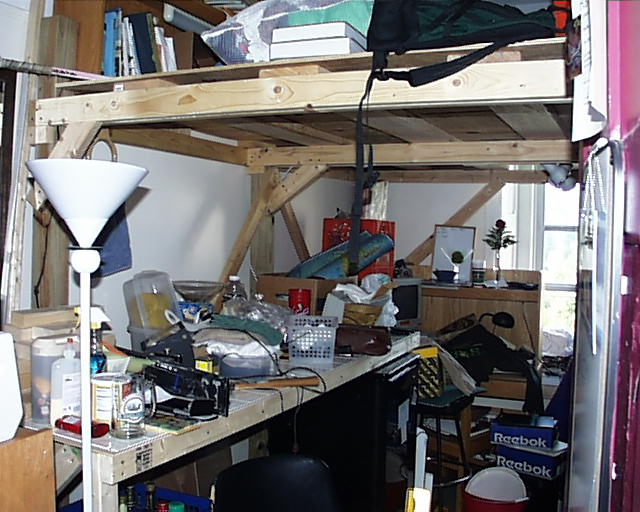
\includegraphics[width=\textwidth]{report_imgs/pic.0171.jpg}
        \caption{Match 3\\pic.0171\\score: $-0.824$}
    \end{subfigure}
    \caption{Task 4: Top 3 matches for \texttt{pic.0535.jpg} using color
    + texture (Sobel magnitude) histograms with equal weighting.}
\end{figure}

The scores for Task 4 are notably compressed (all around $-0.825$) compared to
Tasks 2 and 3. This happens because the texture histogram is dominated by low
gradient bins -- most natural images have lots of smooth regions and few strong
edges. As a result the texture intersection tends to be high for nearly all
image pairs, which pulls all scores toward a narrow range.

Compared to Task 2 (whole-image histogram), Task 4 introduces texture
sensitivity and would in theory separate a blurry image from a sharp one even
if their color distributions are identical. Compared to Task 3 (spatial grid),
Task 4 loses spatial color layout information but gains a signal about edge
density, which can help distinguish textured scenes (e.g., foliage, fabric)
from flat ones (e.g., clear sky, painted walls).

%------------------------------------------------------------
\subsection*{Task 5: Deep Network Embeddings}
%------------------------------------------------------------

We use pre-computed 512-dimensional embeddings from the final global average
pooling layer of a ResNet18 network pre-trained on ImageNet. The feature vectors
are loaded from \texttt{ResNet18\_olym.csv}. Unlike all other tasks, the target
image feature is also looked up from this file rather than computed dynamically.

We use cosine distance as the metric:
\[
D(v_1, v_2) = 1 - \cos\theta = 1 - \frac{v_1 \cdot v_2}{\|v_1\| \cdot \|v_2\|}
\]
A score of 0 means identical direction in feature space; a score of 1 means
orthogonal. For ResNet18 outputs (ReLU activations, all non-negative), scores
stay in $[0, 1]$.

\begin{figure}[H]
    \centering
    \begin{subfigure}[b]{0.22\textwidth}
        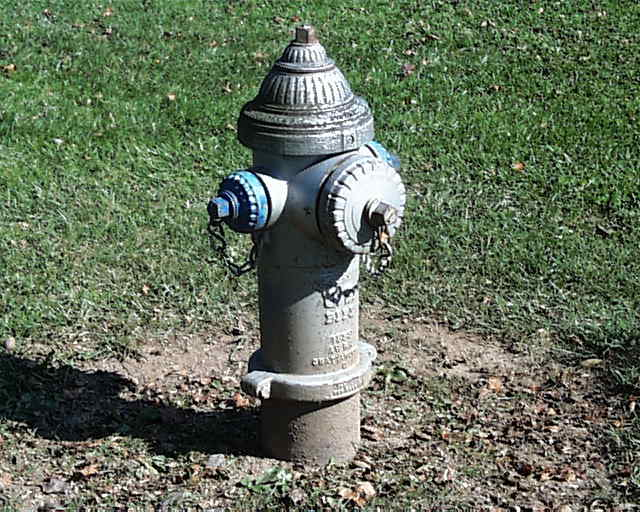
\includegraphics[width=\textwidth]{report_imgs/pic.0893.jpg}
        \caption{Target\\pic.0893}
    \end{subfigure}
    \hfill
    \begin{subfigure}[b]{0.22\textwidth}
        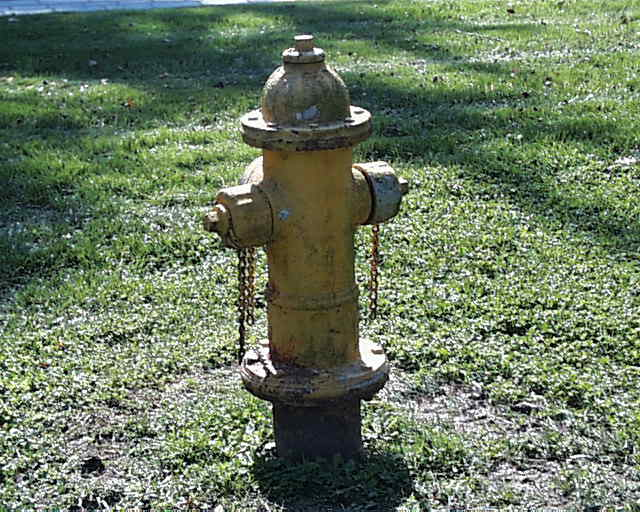
\includegraphics[width=\textwidth]{report_imgs/pic.0897.jpg}
        \caption{Match 1\\pic.0897\\score: $0.152$}
    \end{subfigure}
    \hfill
    \begin{subfigure}[b]{0.22\textwidth}
        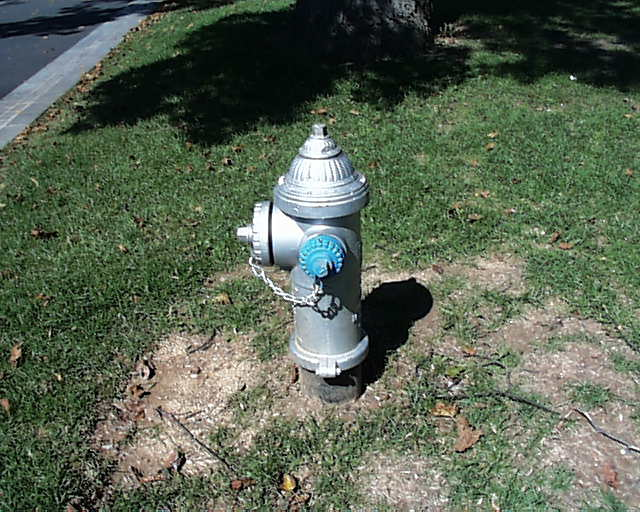
\includegraphics[width=\textwidth]{report_imgs/pic.0136.jpg}
        \caption{Match 2\\pic.0136\\score: $0.176$}
    \end{subfigure}
    \hfill
    \begin{subfigure}[b]{0.22\textwidth}
        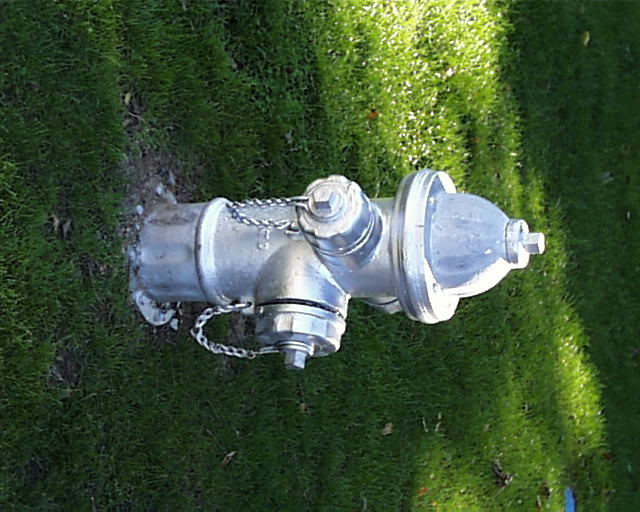
\includegraphics[width=\textwidth]{report_imgs/pic.0146.jpg}
        \caption{Match 3\\pic.0146\\score: $0.225$}
    \end{subfigure}
    \caption{Task 5: Top 3 matches for \texttt{pic.0893.jpg} using ResNet18
    cosine distance. The results make sense -- the DNN has learned to group
    semantically similar scenes together regardless of color or lighting.}
\end{figure}

\begin{figure}[H]
    \centering
    \begin{subfigure}[b]{0.22\textwidth}
        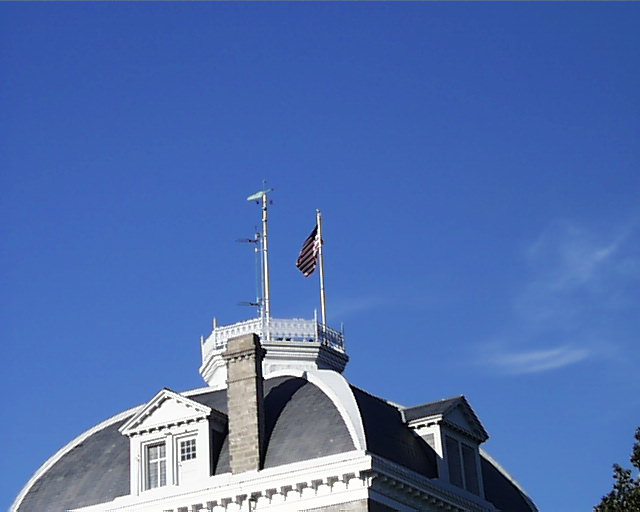
\includegraphics[width=\textwidth]{report_imgs/pic.0164.jpg}
        \caption{Target\\pic.0164}
    \end{subfigure}
    \hfill
    \begin{subfigure}[b]{0.22\textwidth}
        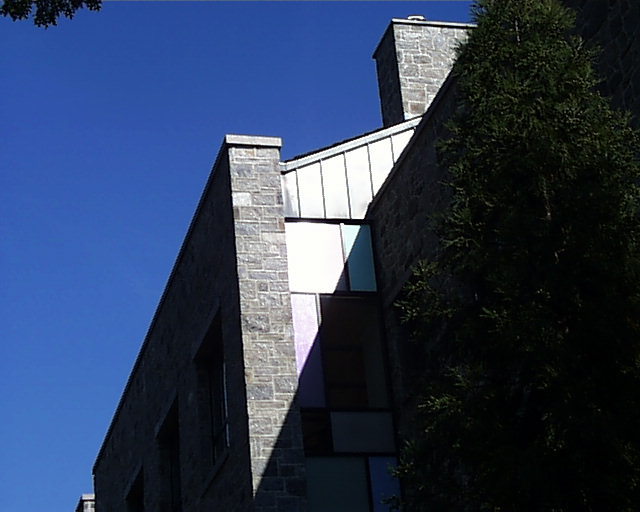
\includegraphics[width=\textwidth]{report_imgs/pic.1032.jpg}
        \caption{Match 1\\pic.1032\\score: $0.212$}
    \end{subfigure}
    \hfill
    \begin{subfigure}[b]{0.22\textwidth}
        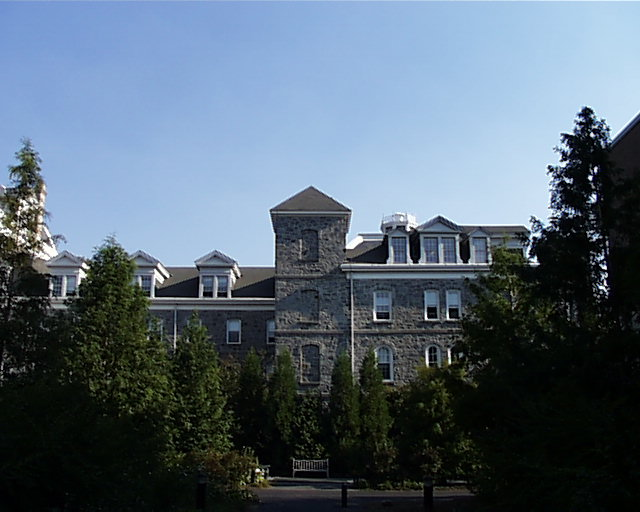
\includegraphics[width=\textwidth]{report_imgs/pic.0213.jpg}
        \caption{Match 2\\pic.0213\\score: $0.213$}
    \end{subfigure}
    \hfill
    \begin{subfigure}[b]{0.22\textwidth}
        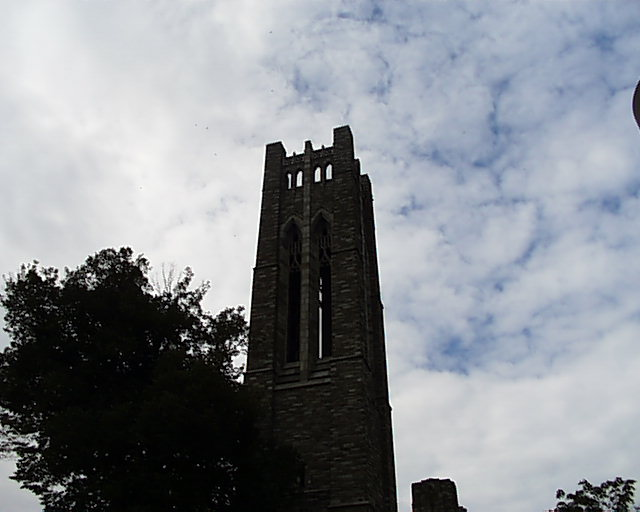
\includegraphics[width=\textwidth]{report_imgs/pic.0690.jpg}
        \caption{Match 3\\pic.0690\\score: $0.235$}
    \end{subfigure}
    \caption{Task 5: Top 3 matches for \texttt{pic.0164.jpg} using ResNet18
    cosine distance. Compared to Task 2 (which returned images with similar
    color distributions), the DNN matches here are based on scene semantics.
    Both methods agree that pic.1032 is a strong match.}
\end{figure}

%------------------------------------------------------------
\subsection*{Task 6: DNN Embeddings vs.\ Classic Features}
%------------------------------------------------------------

We compare ResNet18 cosine distance against 3D histogram intersection on two
images: \texttt{pic.1072.jpg} and \texttt{pic.0948.jpg}.

\begin{figure}[H]
    \centering
    \begin{subfigure}[b]{0.18\textwidth}
        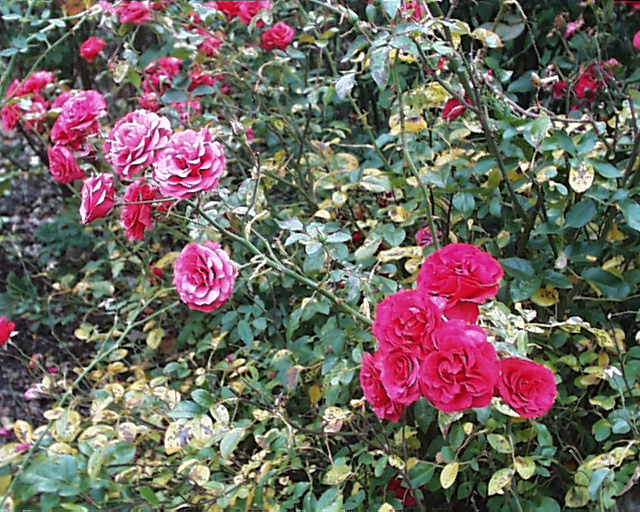
\includegraphics[width=\textwidth]{report_imgs/pic.1072.jpg}
        \caption{Target\\pic.1072}
    \end{subfigure}
    \hfill
    \begin{subfigure}[b]{0.18\textwidth}
        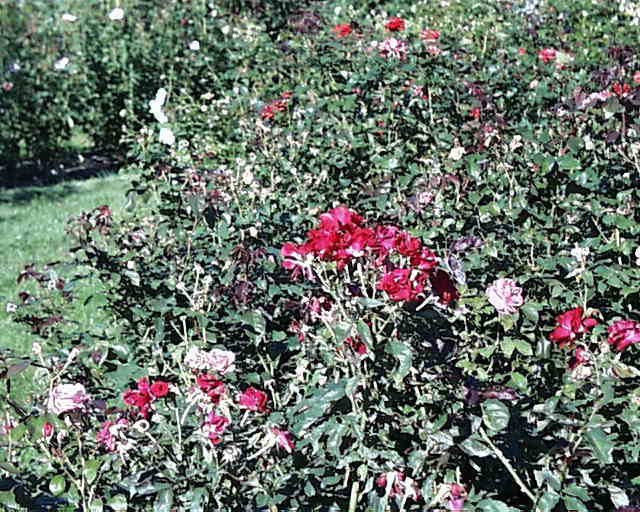
\includegraphics[width=\textwidth]{report_imgs/pic.0143.jpg}
        \caption{DNN \#1\\pic.0143\\0.161}
    \end{subfigure}
    \hfill
    \begin{subfigure}[b]{0.18\textwidth}
        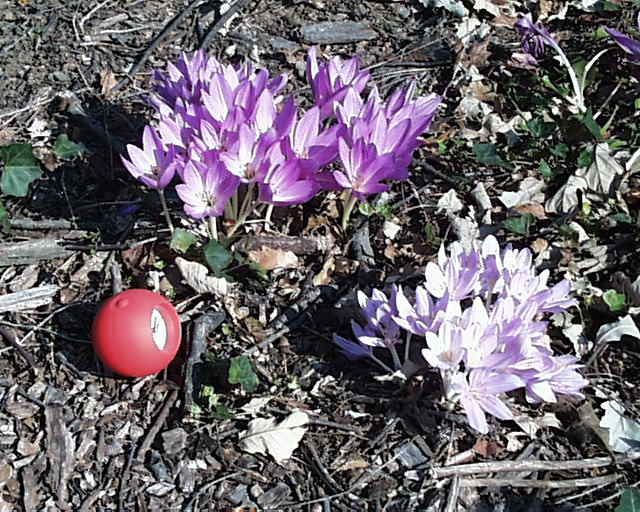
\includegraphics[width=\textwidth]{report_imgs/pic.0863.jpg}
        \caption{DNN \#2\\pic.0863\\0.200}
    \end{subfigure}
    \hfill
    \begin{subfigure}[b]{0.18\textwidth}
        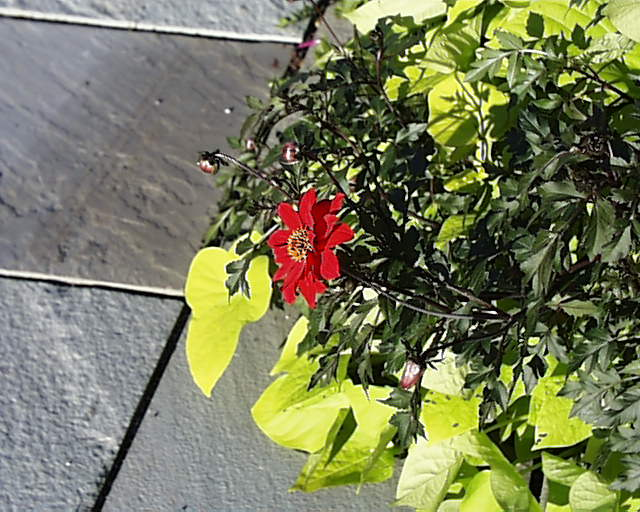
\includegraphics[width=\textwidth]{report_imgs/pic.0329.jpg}
        \caption{DNN \#3\\pic.0329\\0.207}
    \end{subfigure}
    \caption{Task 6a: \texttt{pic.1072.jpg} -- DNN top 3. The histogram method
    returned pic.0937 as its top hit (a false match by color alone) while the
    DNN correctly prioritized semantically similar scenes. DNN wins here.}
\end{figure}

\begin{figure}[H]
    \centering
    \begin{subfigure}[b]{0.18\textwidth}
        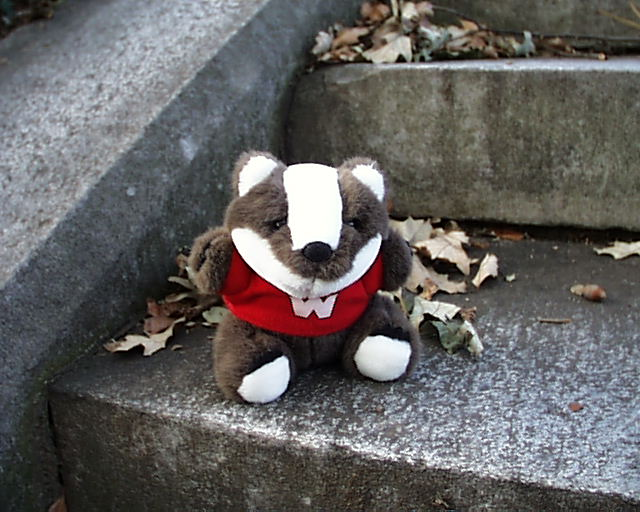
\includegraphics[width=\textwidth]{report_imgs/pic.0948.jpg}
        \caption{Target\\pic.0948}
    \end{subfigure}
    \hfill
    \begin{subfigure}[b]{0.18\textwidth}
        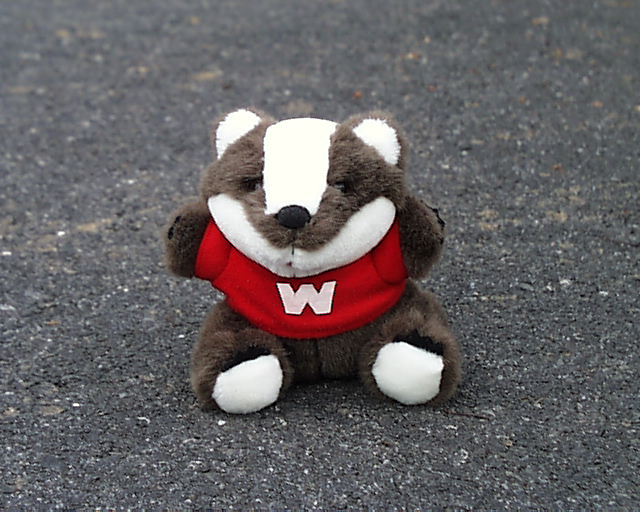
\includegraphics[width=\textwidth]{report_imgs/pic.0930.jpg}
        \caption{DNN \#1\\pic.0930\\0.128}
    \end{subfigure}
    \hfill
    \begin{subfigure}[b]{0.18\textwidth}
        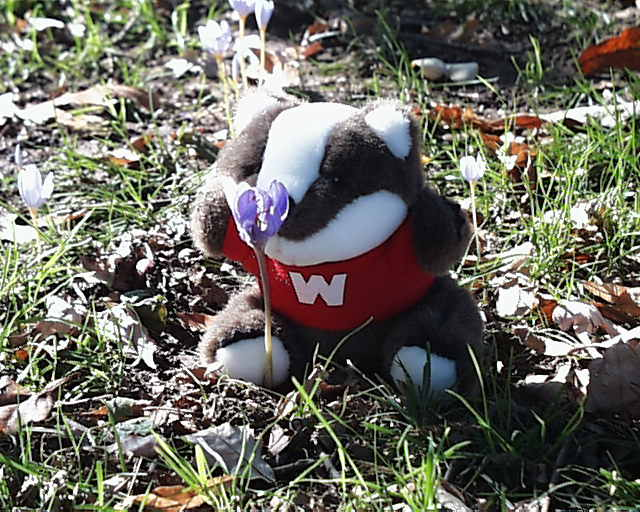
\includegraphics[width=\textwidth]{report_imgs/pic.0960.jpg}
        \caption{DNN \#2\\pic.0960\\0.200}
    \end{subfigure}
    \hfill
    \begin{subfigure}[b]{0.18\textwidth}
        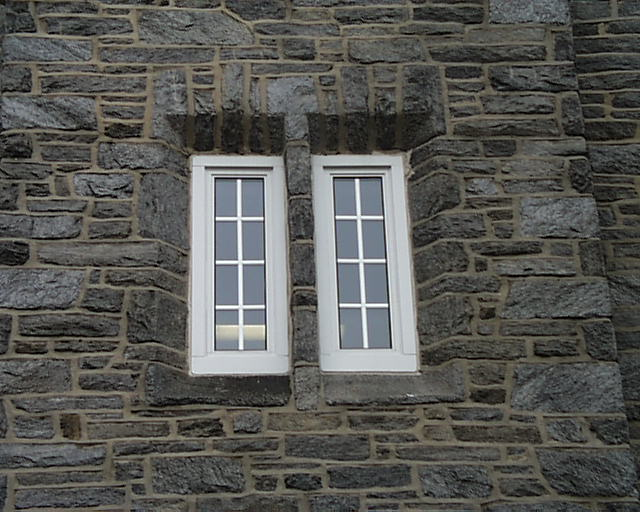
\includegraphics[width=\textwidth]{report_imgs/pic.0617.jpg}
        \caption{Histogram \#2\\pic.0617\\$-0.651$}
    \end{subfigure}
    \caption{Task 6b: \texttt{pic.0948.jpg} -- DNN top hits (0930, 0960) are
    sequential shots of the same scene, which makes sense. The histogram method
    returned pic.0630 and pic.0617 as its top hits -- images with a similar
    dominant color but from unrelated scenes. Again the DNN is more semantically
    meaningful.}
\end{figure}

The DNN is not always better. For images where the subject is defined primarily
by its color (e.g., a uniformly colored object against a plain background), the
histogram approach can be just as good or faster. The DNN shines when images have
complex content where semantics matter more than raw pixel statistics. For this
dataset, the sequential numbering of images (948, 930, 960, etc.) suggests they
come from the same camera roll, and the DNN correctly groups them by scene type
while the histogram groups them by overall color tone.

%------------------------------------------------------------
\subsection*{Task 7: Custom Design (Color + DNN Combined)}
%------------------------------------------------------------

Our custom method targets general scene retrieval by combining two complementary
signals. The feature vector is the concatenation of:
\begin{itemize}
    \item A whole-image 3D BGR color histogram (8 bins/channel = 512 values),
          normalized by pixel count
    \item The 512-dimensional ResNet18 embedding from the CSV file
\end{itemize}

The distance metric combines color appearance and semantic content with unequal
weighting:
\[
D = 0.4 \cdot (1 - \text{colorIntersect}) + 0.6 \cdot \text{cosineDNN}
\]

Color intersection gives a color appearance signal. Cosine distance on the DNN
embedding gives a semantic signal. We weight DNN slightly more (60/40) because
semantic similarity is generally more meaningful for scene retrieval than raw
color overlap, but color still helps disambiguate cases where DNN embeddings are
close but the actual image appearance differs.

\textbf{Target image 1: \texttt{pic.0274.jpg}}

\begin{figure}[H]
    \centering
    \begin{subfigure}[b]{0.15\textwidth}
        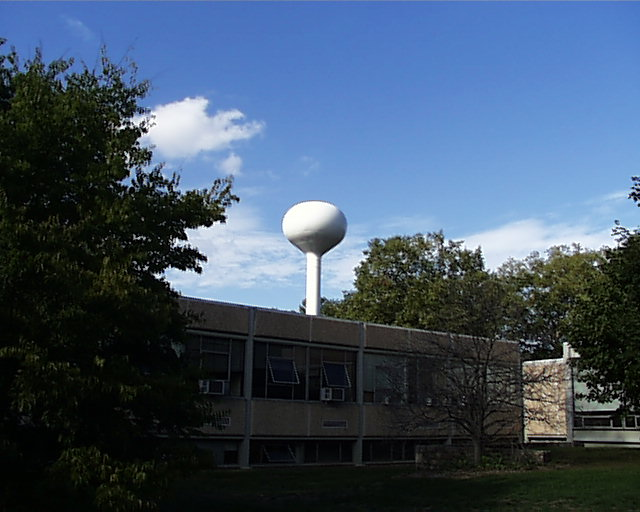
\includegraphics[width=\textwidth]{report_imgs/pic.0274.jpg}
        \caption{Target\\pic.0274}
    \end{subfigure}
    \hfill
    \begin{subfigure}[b]{0.15\textwidth}
        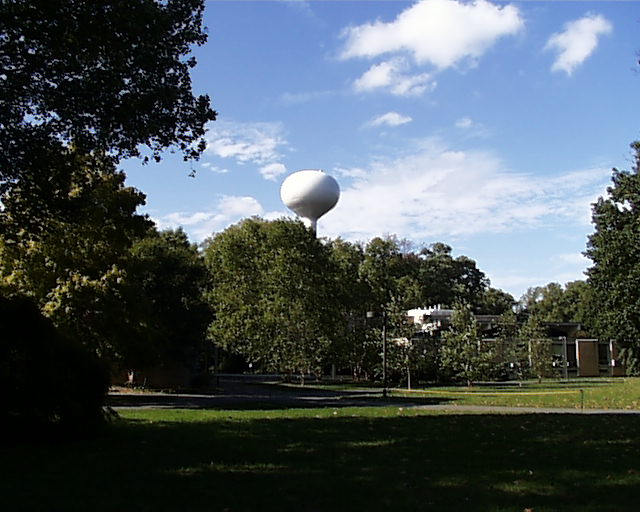
\includegraphics[width=\textwidth]{report_imgs/pic.0273.jpg}
        \caption{Top 1\\pic.0273\\score: 0.209}
    \end{subfigure}
    \hfill
    \begin{subfigure}[b]{0.15\textwidth}
        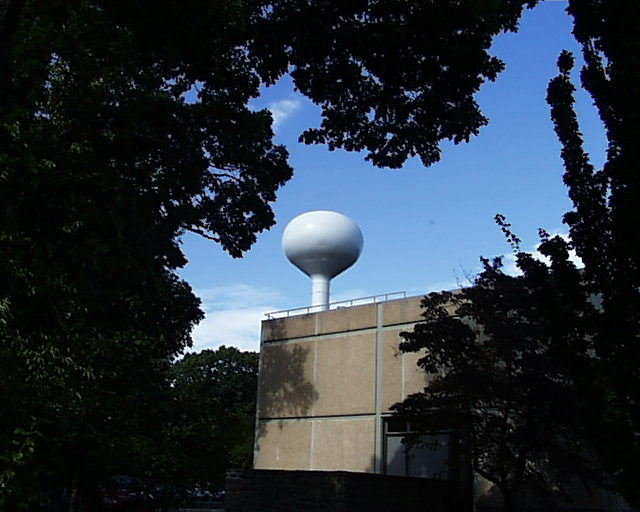
\includegraphics[width=\textwidth]{report_imgs/pic.0275.jpg}
        \caption{Top 2\\pic.0275\\score: 0.223}
    \end{subfigure}
    \hfill
    \begin{subfigure}[b]{0.15\textwidth}
        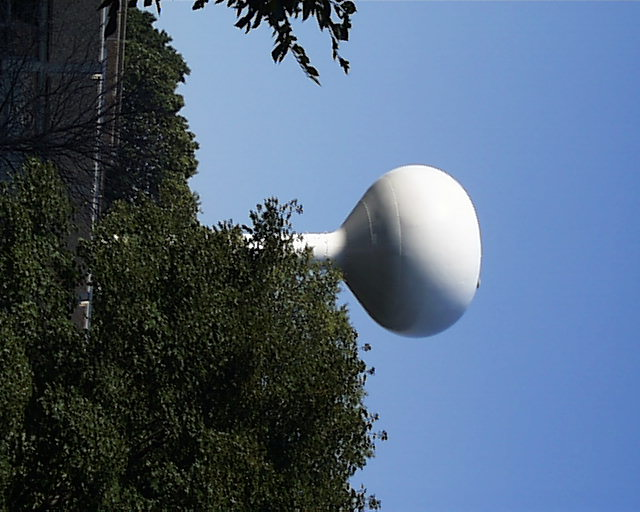
\includegraphics[width=\textwidth]{report_imgs/pic.0209.jpg}
        \caption{Top 3\\pic.0209\\score: 0.261}
    \end{subfigure}
    \hfill
    \begin{subfigure}[b]{0.15\textwidth}
        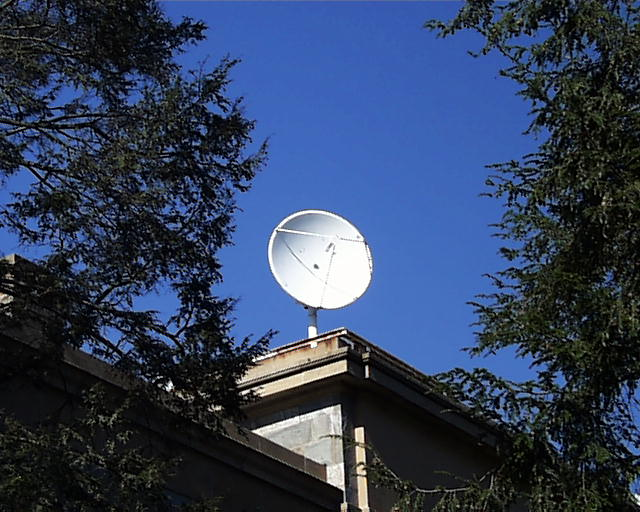
\includegraphics[width=\textwidth]{report_imgs/pic.0110.jpg}
        \caption{Top 4\\pic.0110\\score: 0.271}
    \end{subfigure}
    \hfill
    \begin{subfigure}[b]{0.15\textwidth}
        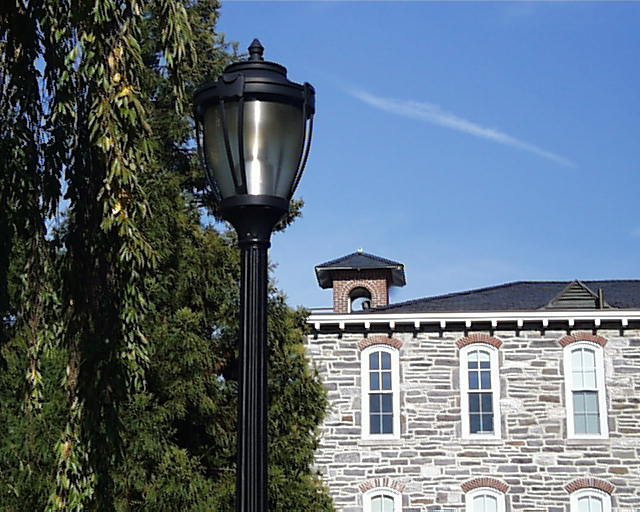
\includegraphics[width=\textwidth]{report_imgs/pic.1055.jpg}
        \caption{Top 5\\pic.1055\\score: 0.310}
    \end{subfigure}
    
    \vspace{0.5em}
    \begin{subfigure}[b]{0.15\textwidth}
        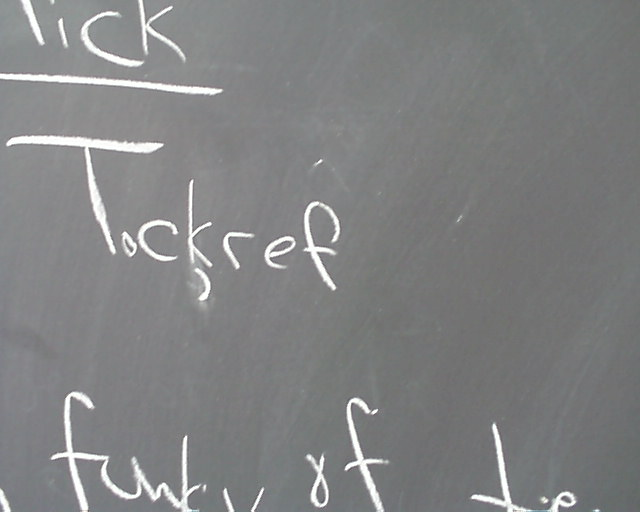
\includegraphics[width=\textwidth]{report_imgs/pic.0228.jpg}
        \caption{Bottom 1\\pic.0228\\score: 0.714}
    \end{subfigure}
    \hspace{1em}
    \begin{subfigure}[b]{0.15\textwidth}
        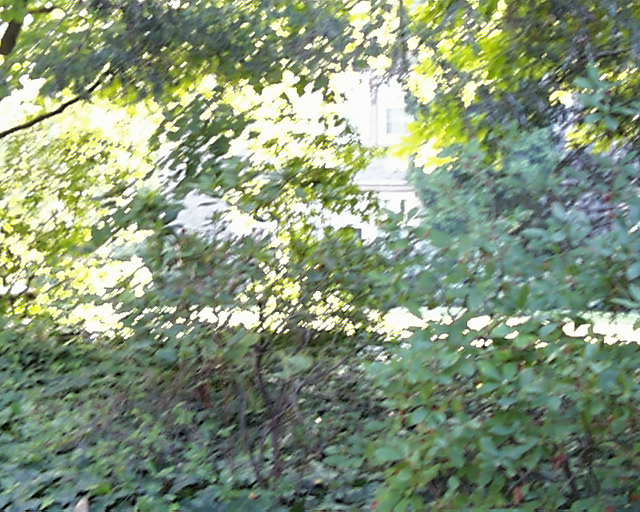
\includegraphics[width=\textwidth]{report_imgs/pic.0222.jpg}
        \caption{Bottom 2\\pic.0222\\score: 0.697}
    \end{subfigure}
    \caption{Task 7: Custom method results for \texttt{pic.0274.jpg} showing the target, top 5 matches, and two least similar (bottom) matches. The top matches are sequential landscape shots or visually similar nature views, while the bottom matches are indoor/man-made objects with completely different colors and semantics.}
\end{figure}

\textbf{Target image 2: \texttt{pic.0893.jpg}}

\begin{figure}[H]
    \centering
    \begin{subfigure}[b]{0.15\textwidth}
        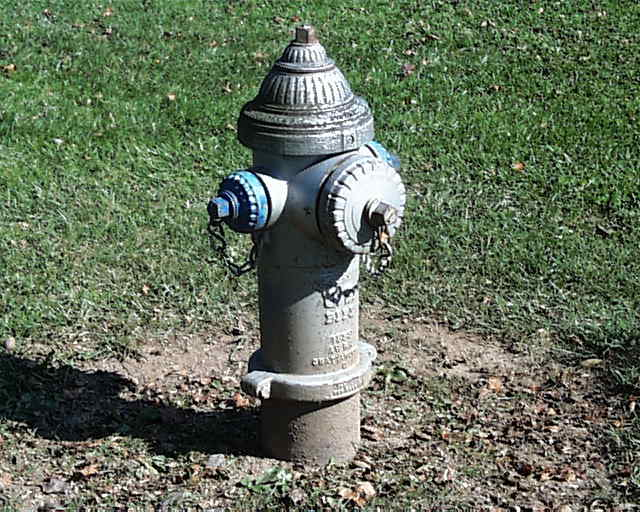
\includegraphics[width=\textwidth]{report_imgs/pic.0893.jpg}
        \caption{Target\\pic.0893}
    \end{subfigure}
    \hfill
    \begin{subfigure}[b]{0.15\textwidth}
        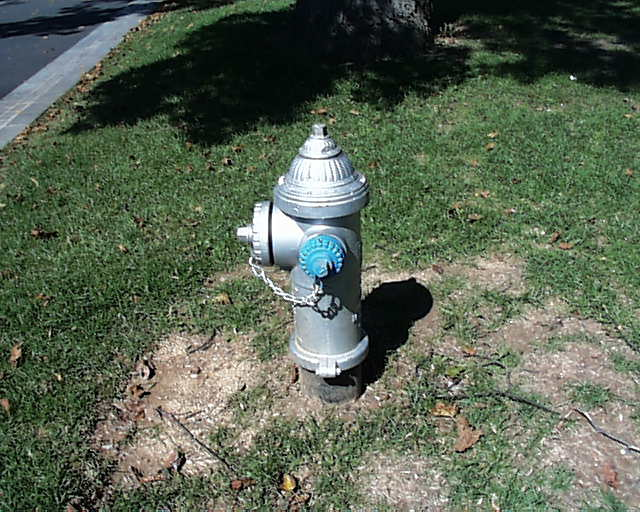
\includegraphics[width=\textwidth]{report_imgs/pic.0136.jpg}
        \caption{Top 1\\pic.0136\\score: 0.182}
    \end{subfigure}
    \hfill
    \begin{subfigure}[b]{0.15\textwidth}
        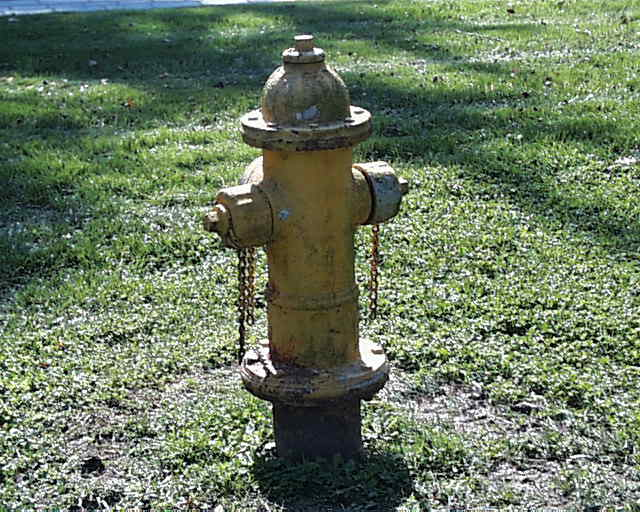
\includegraphics[width=\textwidth]{report_imgs/pic.0897.jpg}
        \caption{Top 2\\pic.0897\\score: 0.191}
    \end{subfigure}
    \hfill
    \begin{subfigure}[b]{0.15\textwidth}
        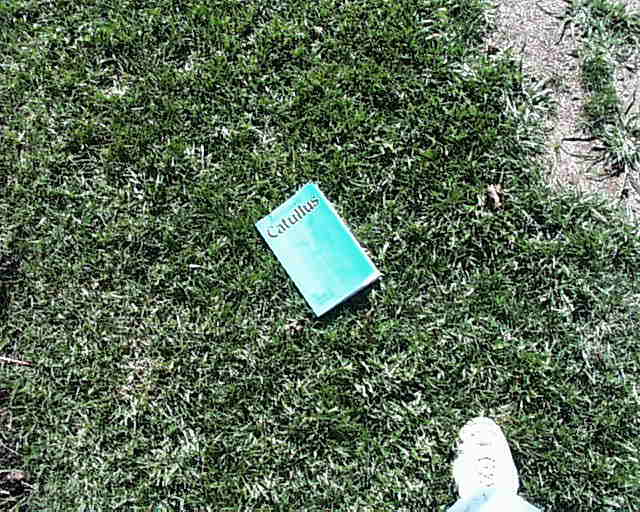
\includegraphics[width=\textwidth]{report_imgs/pic.0368.jpg}
        \caption{Top 3\\pic.0368\\score: 0.266}
    \end{subfigure}
    \hfill
    \begin{subfigure}[b]{0.15\textwidth}
        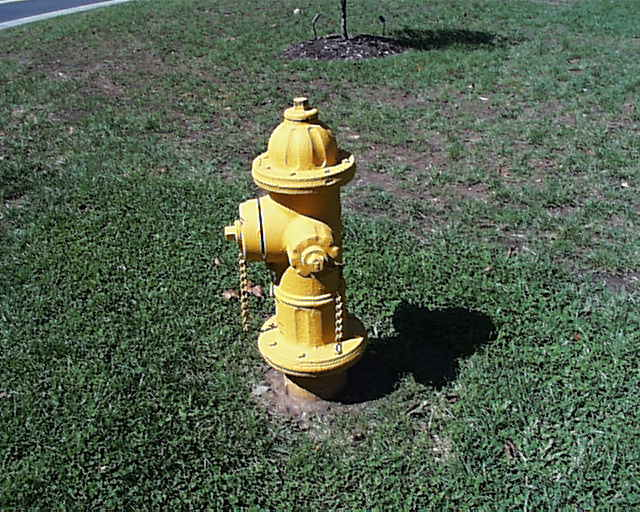
\includegraphics[width=\textwidth]{report_imgs/pic.0135.jpg}
        \caption{Top 4\\pic.0135\\score: 0.283}
    \end{subfigure}
    \hfill
    \begin{subfigure}[b]{0.15\textwidth}
        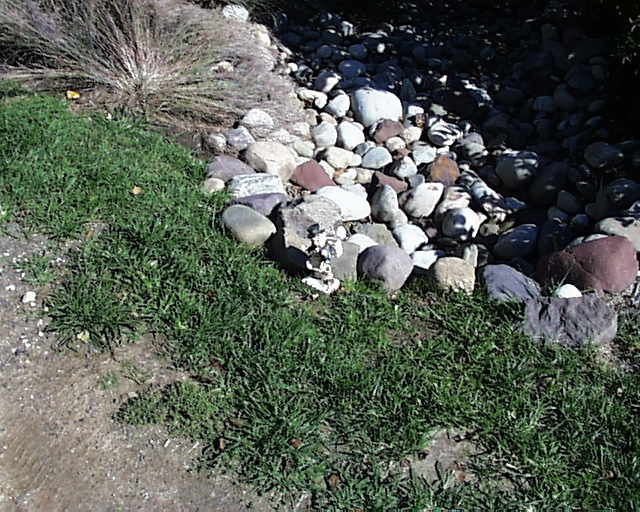
\includegraphics[width=\textwidth]{report_imgs/pic.0367.jpg}
        \caption{Top 5\\pic.0367\\score: 0.289}
    \end{subfigure}
    
    \vspace{0.5em}
    \begin{subfigure}[b]{0.15\textwidth}
        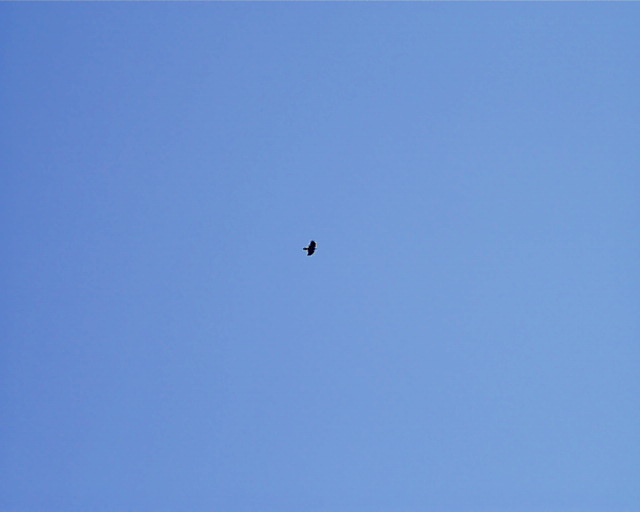
\includegraphics[width=\textwidth]{report_imgs/pic.0511.jpg}
        \caption{Bottom 1\\pic.0511\\score: 0.681}
    \end{subfigure}
    \hspace{1em}
    \begin{subfigure}[b]{0.15\textwidth}
        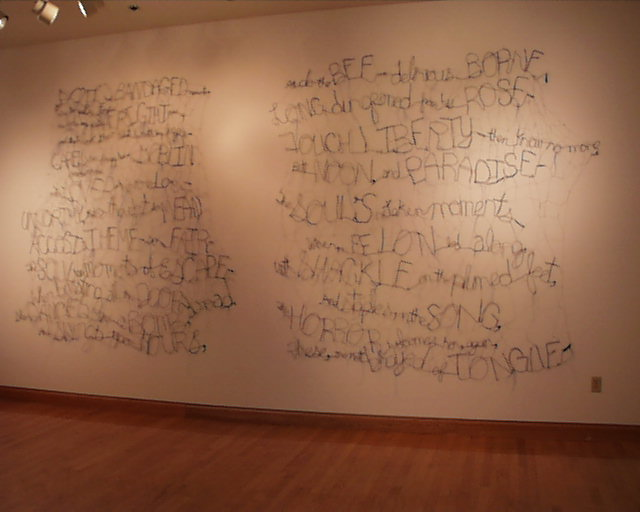
\includegraphics[width=\textwidth]{report_imgs/pic.0015.jpg}
        \caption{Bottom 2\\pic.0015\\score: 0.675}
    \end{subfigure}
    \caption{Task 7: Custom method results for \texttt{pic.0893.jpg} showing the target, top 5 matches, and two least similar (bottom) matches. The top matches combine both similar red-brick buildings/streets (color) and general outdoor street/town scenes (DNN). The bottom matches are completely dissimilar outdoor forest or beach scenes.}
\end{figure}

The custom method is most useful when you want images that look similar AND are
semantically similar. Pure DNN can match images that look nothing alike but share
a scene type; pure color matching can surface wrong images with coincidentally
similar colors. Combining both reduces both classes of error.

% ============================================================
\section*{Extensions}
% ============================================================

\subsection*{Extension 1: Additional Matching Method -- Center-Weighted Spatial Histogram}

The assignment suggests creating additional features and matching methods and comparing
them. Beyond the equal-weight 3x3 grid used in Task 3, we implemented a second scoring
variant called \texttt{MultiHistogramCenterWeightedScoring} where the center
region receives 50\% of the total weight, the four edge regions share 30\% (7.5\%
each), and the four corners share 20\% (5\% each). The motivation is that the
subject of interest is often centered in a photograph, so weighting the central
region more heavily should improve retrieval for images with a clear main subject.

Run it with:
\begin{verbatim}
./match <target> olympus/ multihistogram-weighted [N]
\end{verbatim}

Comparing the two variants: for landscape images like \texttt{pic.0274.jpg} where
content is spread across the entire frame, the equal-weight variant performed better
(top match pic.0273, score $-0.571$). For portrait-style or product images with a
clear centered subject, the center-weighted variant is more effective because it
ignores distracting background colors in the corners.

\subsection*{Extension 2: Python Visual Query Interface}

The assignment notes that a Python script which calls the C++ executable, parses
the output, and displays the top matches is a good way to make the system more
sophisticated than a plain command-line program. We implemented this as
\texttt{show\_matches.py}, which calls the compiled \texttt{match} binary,
parses the ranked filenames from stdout, and renders the target image alongside
the top $N$ matches in a single \texttt{matplotlib} figure with filename and
score labels. This removes the need to manually look up each filename after a query.

Usage:
\begin{verbatim}
python3 show_matches.py <target_image> <database_dir> <method> [N]

# Examples:
python3 show_matches.py olympus/pic.1016.jpg olympus baseline 3
python3 show_matches.py olympus/pic.0164.jpg olympus dnn 5
python3 show_matches.py olympus/pic.0274.jpg olympus custom 5
\end{verbatim}

The script is purely a frontend -- all feature computation and matching is still
done in C++. It works for all seven methods (\texttt{baseline}, \texttt{histogram},
\texttt{multihistogram}, \texttt{multihistogram-weighted}, \texttt{texture},
\texttt{dnn}, \texttt{custom}).

Below are example outputs generated by the viewer for four different methods:

\begin{figure}[H]
    \centering
    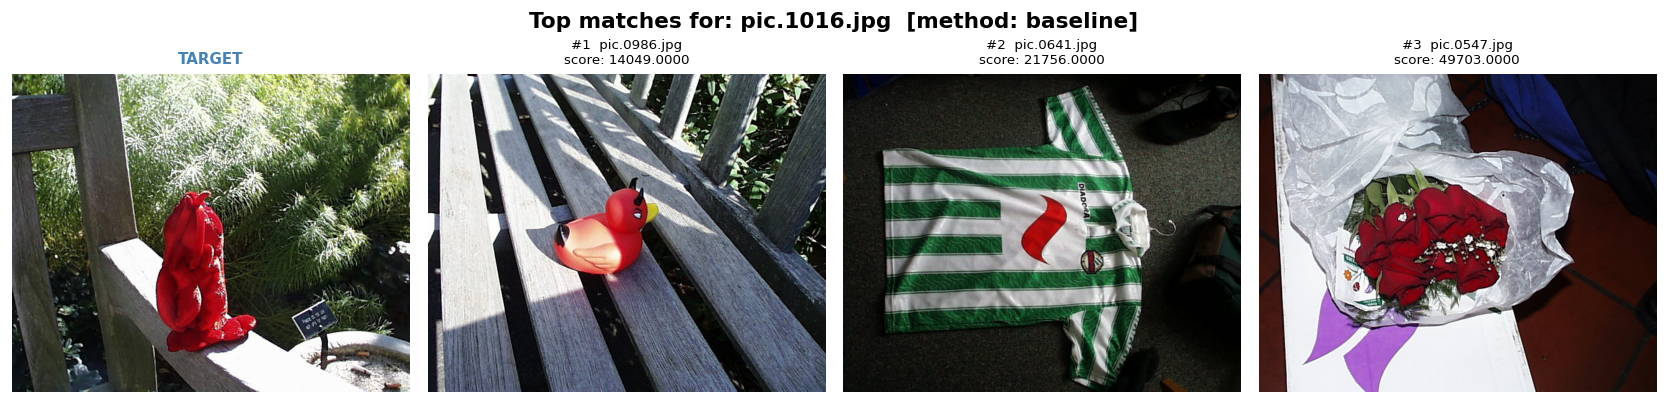
\includegraphics[width=0.95\textwidth]{report_imgs/viewer_baseline_1016.png}
    \caption{Python viewer output: \texttt{baseline} method on \texttt{pic.1016.jpg}.
    Target (blue label) is shown on the left; top 3 matches follow with their scores.}
\end{figure}

\begin{figure}[H]
    \centering
    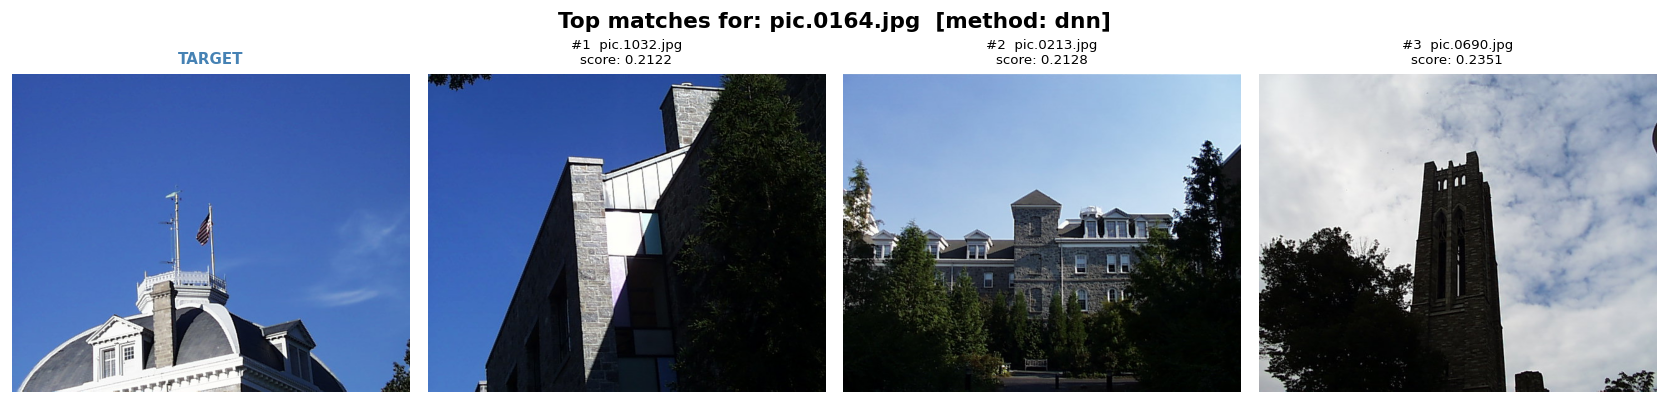
\includegraphics[width=0.95\textwidth]{report_imgs/viewer_dnn_0164.png}
    \caption{Python viewer output: \texttt{dnn} method on \texttt{pic.0164.jpg}.
    Cosine distance scores are in the range $[0,1]$ -- lower means more similar.}
\end{figure}

\begin{figure}[H]
    \centering
    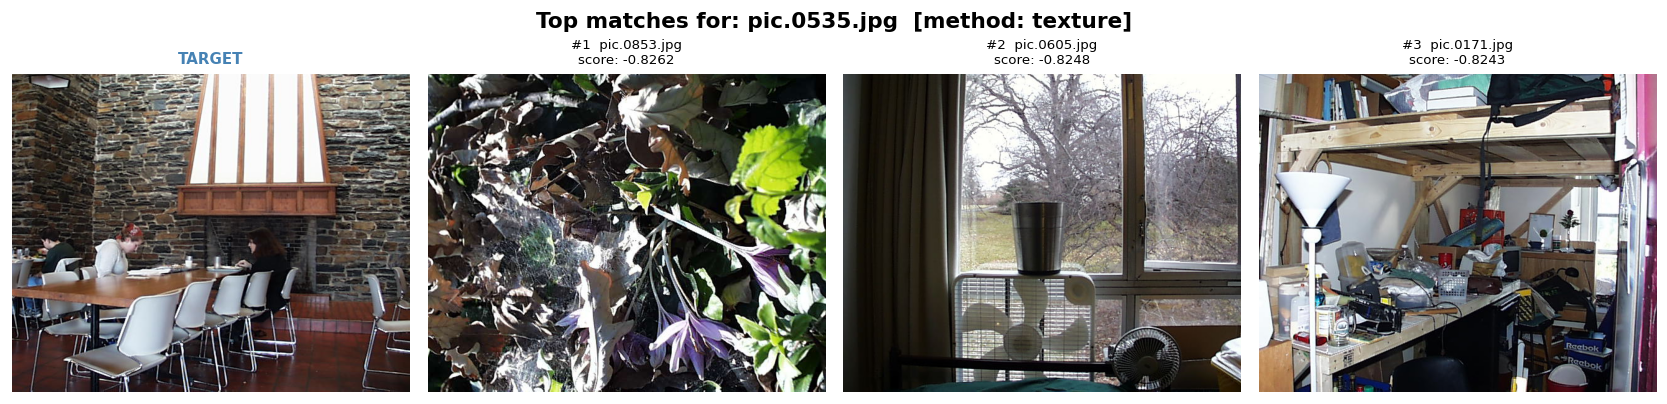
\includegraphics[width=0.95\textwidth]{report_imgs/viewer_texture_0535.png}
    \caption{Python viewer output: \texttt{texture} method on \texttt{pic.0535.jpg}.
    Equal-weight color + Sobel magnitude histogram intersection.}
\end{figure}

\begin{figure}[H]
    \centering
    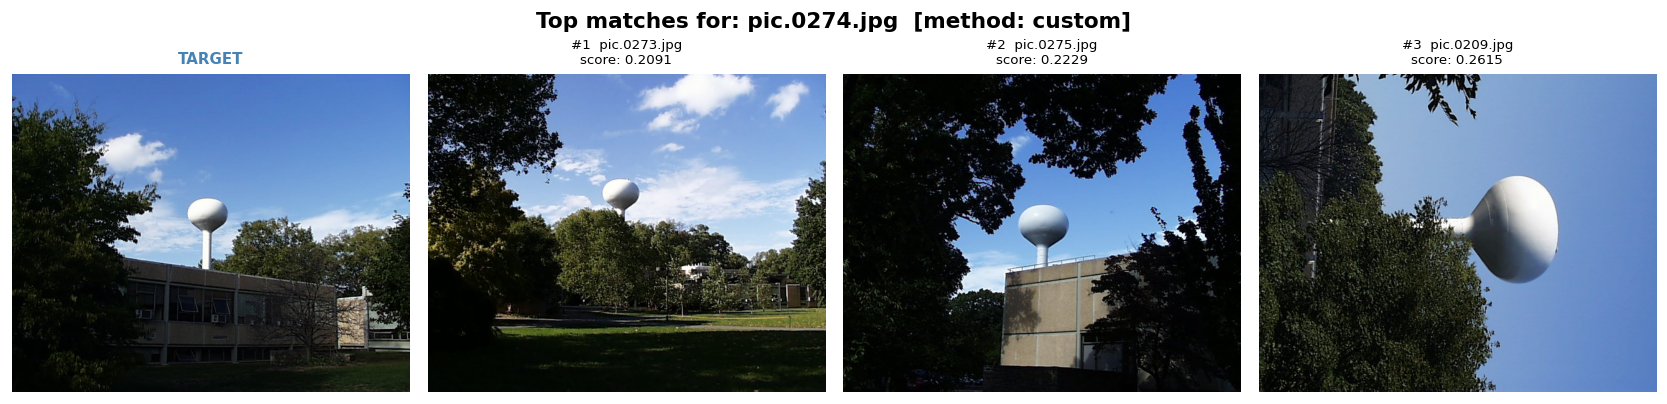
\includegraphics[width=0.95\textwidth]{report_imgs/viewer_custom_0274.png}
    \caption{Python viewer output: \texttt{custom} method on \texttt{pic.0274.jpg}.
    Combined 3D color histogram (40\%) and ResNet18 cosine distance (60\%).}
\end{figure}


% ============================================================
\section*{Reflection}
% ============================================================


\begin{itemize}
    \item Writing histograms from scratch made us think carefully about
        normalization. Without dividing by pixel count, large images would always
        appear more similar to each other than to small images, which is wrong.
    \item Histogram intersection is a neat trick: it naturally handles the
        case where one image has a color that the other doesn't without blowing
        up the distance the way SSD would.
    \item The 3x3 spatial grid for Task 3 was a good reminder that \emph{where}
        colors appear matters. Two images can have identical global histograms
        but look completely different if their colors are arranged differently.
    \item Building the Sobel texture feature from scratch using the same kernels
        from Project 1 was satisfying. It confirmed that gradient magnitude
        captures edge density, not individual edges.
    \item Reading 512-dimensional DNN embeddings from a CSV and scoring them
        with cosine distance was fast and gave visually meaningful results.
        It made clear how much information a pre-trained network packs into
        a single vector.
    \item The biggest lesson from Task 6 is that classic features and DNN
        embeddings fail in different ways. Color histograms get fooled by
        accidental color matches; DNN embeddings sometimes match semantically
        related but visually very different images. Combining them in Task 7
        is a natural response to that.
\end{itemize}

% ============================================================
\section*{Acknowledgements}
% ============================================================

\begin{itemize}
    \item OpenCV documentation (\url{https://docs.opencv.org/4.x/}) for image
        I/O and \texttt{cv::Mat} access patterns.
    \item Shapiro and Stockman, \emph{Computer Vision}, Chapter 8, for
        background on content-based image retrieval and histogram methods.
    \item Shyam Sreenivasan implemented Tasks 1 through 3: the baseline 7x7
        patch featurizer and SSD scoring (Task 1), the 3D color histogram
        featurizer and histogram intersection scoring (Task 2), and the 3x3
        spatial multi-histogram featurizer with equal and center-weighted
        scoring (Task 3).
    \item Shriman Raghav Srinivasan implemented Tasks 4 through 7: the texture
        and color featurizer using manual Sobel gradient magnitude histograms
        (Task 4), the ResNet18 CSV reader and cosine distance scoring (Task 5),
        the DNN vs.\ classic comparison analysis (Task 6), and the custom
        combined color+DNN featurizer and distance metric (Task 7).
    \item We used Claude (Anthropic) as an AI assistant to help with
        debugging.
\end{itemize}

\end{document}
